% ============================================================
% EEEC 1099 Biomedical Sensors - Spring 2026
% HW5 Lab Report (Resubmission)
% Compact lab-report-style article. Source figures live in ../outputs/figures/.
% ============================================================
\documentclass[11pt,a4paper]{article}

\usepackage[margin=0.9in]{geometry}
\usepackage{graphicx}
\usepackage{booktabs}
\usepackage{caption}
\usepackage{siunitx}
\usepackage{tabularx}
\usepackage{float}
\usepackage{subcaption}
\usepackage[hidelinks]{hyperref}
\usepackage{parskip}

\graphicspath{{../outputs/figures/}}

\sisetup{group-separator={,}}

\captionsetup{font=small,labelfont=bf,skip=4pt}
\captionsetup[subfigure]{font=footnotesize,labelfont=bf,skip=2pt,
  justification=centering,width=0.96\linewidth}

\setlength{\parskip}{0.3em}
\setlength{\parindent}{0pt}

% Tighten section/subsection spacing for a compact lab-report feel.
\makeatletter
\renewcommand\section{\@startsection{section}{1}{\z@}%
  {-1.2ex plus -0.5ex minus -0.2ex}{0.5ex plus 0.2ex}%
  {\normalfont\large\bfseries}}
\renewcommand\subsection{\@startsection{subsection}{2}{\z@}%
  {-0.8ex plus -0.4ex minus -0.2ex}{0.3ex plus 0.2ex}%
  {\normalfont\normalsize\bfseries}}
\makeatother

% Float placement: prefer inline (here/top), keep figures with surrounding text.
\renewcommand{\topfraction}{0.9}
\renewcommand{\bottomfraction}{0.8}
\renewcommand{\floatpagefraction}{0.85}
\setlength{\textfloatsep}{10pt plus 4pt minus 3pt}
\setlength{\intextsep}{10pt plus 4pt minus 3pt}
\setlength{\floatsep}{10pt plus 4pt minus 3pt}
\setlength{\abovecaptionskip}{4pt}

\begin{document}

% --------- Title block ---------
\begin{center}
  {\Large\bfseries HW5 Lab Report:\\[0.2em]
  Single-Lead ECG and Heart Rate Variability under Four Physiological Tasks\par}
  \vspace{0.6em}
  {\normalsize Pei-En Wu\par}
  \vspace{0.2em}
  {\small NYCU ID: 113511103 \quad
   Email: \href{mailto:peienwu.ee13@nycu.edu.tw}{peienwu.ee13@nycu.edu.tw}\\
   Department of Medicine \& Department of Electrical Engineering,
   National Yang Ming Chiao Tung University\par}
  \vspace{0.3em}
  {\footnotesize EEEC~1099 Biomedical Sensors, Spring~2026 \textemdash{}
   HW5 Lab Report\par}
\end{center}

\vspace{0.4em}

% ============================================================
\section{Objective}
This lab characterizes a single-lead chest-patch ECG sensor by quantifying
heart rate (HR) and heart rate variability (HRV) responses under four
physiological tasks: postural baseline (Q1), voluntary breath-hold (Q2),
ambulatory walking (Q3), and a self-designed paced-breathing variation
(Q4). The goal is to relate sensor outputs to known cardiorespiratory
mechanisms and to identify conditions where ECG interpretation requires
caution.

% ============================================================
\section{Apparatus and Subject}
A VitalSigns VS-ECG VSH101 chest-patch sensor recorded single-lead ECG at
500\,Hz and triaxial accelerometry at 25\,Hz on one adult male participant
(age 22, no known cardiovascular or respiratory conditions). All 14
recordings were acquired in a single indoor session on April 24, 2026.
ECG was preprocessed in Python with a two-stage median filter for baseline
correction (200/600\,ms kernels), a 60\,Hz IIR notch ($Q{=}30$), and a
0.5--40\,Hz Butterworth bandpass (zero-phase). R-peak detection used
NeuroKit2 \texttt{ecg\_peaks} with Kubios-style artifact
correction~\cite{makowski2021}, cross-checked against an independent
SciPy Pan--Tompkins detector~\cite{pan1985} (peak-count agreement
$\geq$99.5\% across steady-state sessions).

% ============================================================
\section{Procedure}
\begin{itemize}
\setlength{\itemsep}{0.1em}
\item \textbf{Q1 (E1) Postural baseline.} Three consecutive 5-min
  recordings in supine, sitting, and standing postures with quiet
  spontaneous breathing.
\item \textbf{Q2 (E2) Transpulmonary effects.} Seated 40-s maximum
  inspiratory breath-hold and 40-s maximum expiratory breath-hold, each
  repeated twice with $\geq$1\,min recovery between trials.
\item \textbf{Q3 (E3) Ambulatory recording.} Continuous 180-s recording
  segmented into 60\,s seated baseline, 60\,s self-paced walking, and
  60\,s seated recovery.
\item \textbf{Q4 (E4, self-designed) Paced breathing.} Five seated
  paced-breathing conditions (12, 9, 6, 5, and 3 breaths/min) guided by
  metronome, each lasting 220--280\,s with $\geq$3\,min inter-condition
  rest.
\end{itemize}

% ============================================================
\section{HRV Metrics}

The following heart rate variability (HRV) indices are reported
throughout, following Task Force definitions~\cite{taskforce1996}:

\textbf{Time domain.}
\begin{itemize}\setlength{\itemsep}{0.1em}
\item \textbf{SDNN} --- standard deviation of all normal-to-normal (NN)
  intervals; reflects total variability over the analysis window and is
  strongly duration-dependent~\cite{taskforce1996}.
\item \textbf{RMSSD} --- root mean square of successive NN-interval
  differences; captures short-term beat-to-beat variability driven
  predominantly by vagal modulation~\cite{taskforce1996,shaffer2017}.
  Unlike HF power, RMSSD does not depend directly on fixed spectral-band
  definitions and is therefore less affected by respiratory-band migration
  across the LF/HF boundary.
\item \textbf{pNN50} --- proportion of successive NN pairs differing by
  $>$50\,ms; a parasympathetic-related index highly correlated with RMSSD.
\end{itemize}

\textbf{Frequency domain.}
RR intervals were resampled at 4\,Hz and analysed via Welch PSD (Hann
window, 50\% overlap). Band powers follow the Task Force ranges:
\begin{itemize}\setlength{\itemsep}{0.1em}
\item \textbf{LF} (0.04--0.15\,Hz) --- mixed sympathetic and
  parasympathetic modulation.
\item \textbf{HF} (0.15--0.40\,Hz) --- predominantly vagal modulation,
  typically entrained by respiration at normal breathing rates.
\item \textbf{LF/HF ratio} --- historically used as a
  sympathovagal-balance index, but can be difficult to interpret when the
  respiratory peak falls below 0.15\,Hz (see Q4).
\end{itemize}

% ============================================================
\section{Results}

% ------------------ Q1 ------------------
\subsection{Q1: Postural Baseline}

\begin{table}[H]
\centering
\caption{Postural baseline HRV metrics (5-min windows).}
\label{tab:q1}
\small
\begin{tabular}{@{}lccc@{}}
\toprule
Metric & Supine & Sitting & Standing \\
\midrule
Mean HR (bpm)           & 54.0   & 56.1   & 79.7 \\
SDNN (ms)               & 81.5   & 56.6   & 41.8 \\
RMSSD (ms)              & 99.1   & 61.1   & 25.2 \\
pNN50 (\%)              & 62.2   & 43.5   & 2.8  \\
HF (ms$^{2}$)           & 3256.8 & 1123.4 & 310.9 \\
LF/HF                   & 0.28   & 0.53   & 1.44 \\
\bottomrule
\end{tabular}
\end{table}

\begin{figure}[H]
\centering
\includegraphics[width=0.90\linewidth,height=0.50\textheight,keepaspectratio]%
  {hw05_q1_rr_psd_postural.pdf}
\caption{Representative 100-s RR-interval excerpts (top; y-axis in seconds)
and full-window (300\,s) RR-power spectra (bottom) across the three
postures. Supine shows larger beat-to-beat variability and higher HF
power; standing shows shorter RR intervals and reduced HF.}
\label{fig:q1_rr}
\end{figure}

Orthostatic loading was associated with monotonic changes in HR and HRV
(Table~\ref{tab:q1}). From supine to standing, mean HR increased from
54.0 to 79.7\,bpm and RMSSD fell from 99.1 to 25.2\,ms, consistent with
progressive vagal withdrawal~\cite{taskforce1996}. The RR-interval time
series (Fig.~\ref{fig:q1_rr}, top) showed clear amplitude compression
from supine to standing, and the RR power spectrum (Fig.~\ref{fig:q1_rr},
bottom) showed a respiratory-band peak near 0.22--0.30\,Hz in all three
postures.

The ECG power spectral density (0.05--5\,Hz; Fig.~\ref{fig:q1_ecg_psd})
resolved the cardiac fundamental $f_{0}$ shifting from
0.90\,Hz (supine) and 0.93\,Hz (sitting) to 1.33\,Hz (standing), with
visible harmonics at $2f_{0}$ and $3f_{0}$ in all conditions.
A respiratory-band modulation peak near 0.22--0.30\,Hz appeared in both
ECG- and RR-domain spectra, consistent with a respiratory contribution.

Poincar\'e return maps (Fig.~\ref{fig:q1_poincare}) show the reduction
in beat-to-beat variability across postures: the point cloud contracts
progressively from supine to standing (SD1: 68.3 to 17.9\,ms), consistent
with the RMSSD trend in Table~\ref{tab:q1}.

\begin{figure}[H]
\centering
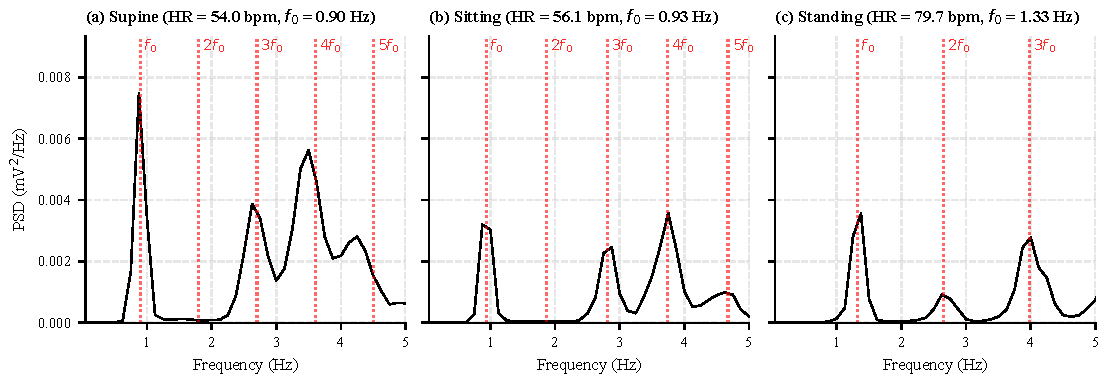
\includegraphics[width=0.92\linewidth]{hw05_q1_ecg_psd_postures_row3.pdf}
\caption{ECG power spectral density across postures. The cardiac
fundamental shifted from 0.90~Hz (supine) to 1.33~Hz (standing).
Harmonic peaks at $2f_{0}$ and $3f_{0}$ are visible across
conditions. Respiratory-band modulation, most prominent in the supine
recording, likely reflects respiratory-related rate modulation.}
\label{fig:q1_ecg_psd}
\end{figure}

\begin{figure}[H]
\centering
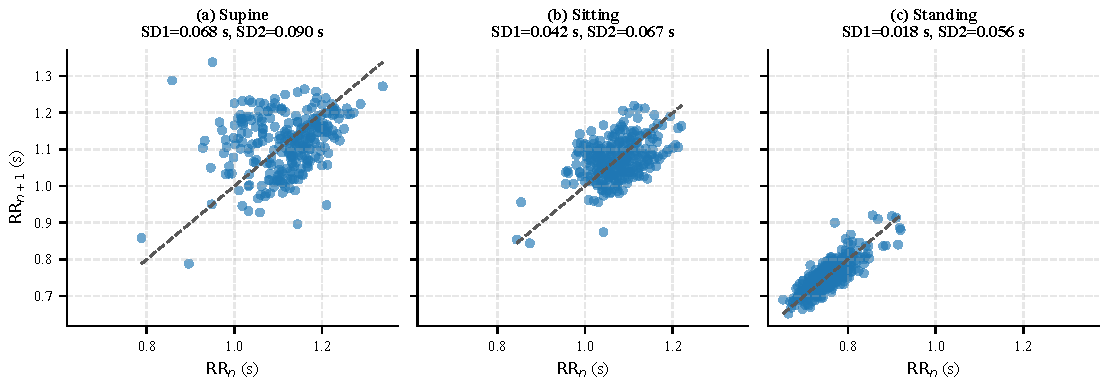
\includegraphics[width=0.92\linewidth]{hw05_q1_poincare_postures_row3.pdf}
\caption{Poincar\'e return maps ($\text{RR}_{n}$ vs.\
$\text{RR}_{n+1}$, in seconds) across the three postures. Each point
represents one consecutive beat pair from the full 5-min recording. The
dashed line is the identity ($\text{RR}_{n+1} = \text{RR}_{n}$). SD1
captures short-term (perpendicular) scatter and SD2 the longer-term
(along-identity) spread. The point cloud contracts progressively from
supine to standing (SD1: 0.068 to 0.018\,s), consistent with declining
vagal modulation.}
\label{fig:q1_poincare}
\end{figure}

% ------------------ Q2 ------------------
\subsection{Q2: Transpulmonary Effects (Breath-Hold)}

\begin{table}[H]
\centering
\caption{Breath-hold trial-level metrics. HF values from the 40-s hold
and recovery windows are reported as descriptive short-window estimates
rather than standard 5-min frequency-domain HRV measures. Spectral HF is
reported for Trial~2 only; Trial~1 was excluded from spectral comparison
because the inspiratory trace was nonstationary.}
\label{tab:q2}
\small
\begin{tabular}{@{}lcccc@{}}
\toprule
 & \multicolumn{2}{c}{Inspiratory} & \multicolumn{2}{c}{Expiratory} \\
\cmidrule(lr){2-3}\cmidrule(lr){4-5}
Metric & Trial~1 & Trial~2 & Trial~1 & Trial~2 \\
\midrule
Pre-hold HR (bpm)      & 62.9   & 59.2 & 58.8 & 58.9 \\
Hold mean HR (bpm)     & 66.9   & 73.5 & 57.8 & 60.8 \\
$\Delta$HR (bpm)       & +4.0   & +14.3 & $-$0.9 & +1.9 \\
HR slope (bpm/s)       & $-$0.19 & +0.18 & $-$0.10 & $-$0.11 \\
Hold HF (ms$^{2}$)     & ---    & 39.1 & ---  & 230.9 \\
Recovery HF (ms$^{2}$) & ---    & 1207 & ---  & 1213 \\
\bottomrule
\end{tabular}
\end{table}

Inspiratory breath-hold produced larger HR responses than expiratory
hold (Table~\ref{tab:q2}). In the relaxed trial (Trial~2), inspiratory
hold raised mean HR by +14.3\,bpm whereas expiratory hold changed HR by
only +1.9\,bpm. This asymmetry may reflect the effect of sustained lung
inflation on intrathoracic pressure and venous return, producing a more
pronounced reflex HR rise. Spectral analysis on the relaxed trial showed
that inspiratory hold reduced HF power to 39.1\,ms$^{2}$ (a $-96.5\%$
change versus the seated anchor of 1123\,ms$^{2}$), compared with
230.9\,ms$^{2}$ ($-79.4\%$) during expiratory hold. Both conditions
recovered toward the seated-anchor HF value within the 50-s post-hold
window, suggesting a transient perturbation rather than a sustained
autonomic shift. Trial-1 data showed substantial inter-trial variability
in the inspiratory condition, possibly reflecting volitional effort or
anticipation during the early effort (Fig.~\ref{fig:q2_breathhold}).

\begin{figure}[H]
\centering
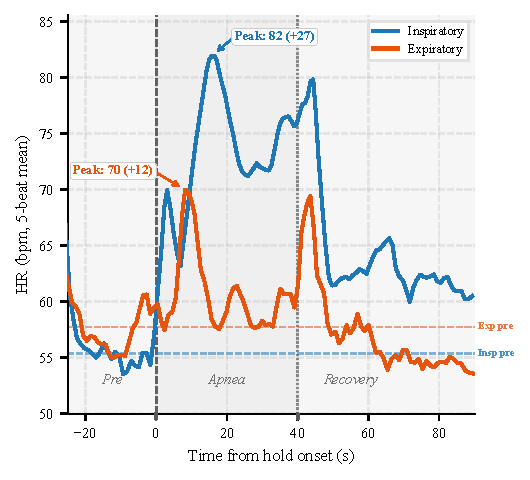
\includegraphics[width=0.70\linewidth]{nb03_fig03_e2_pure_physiology.pdf}
\caption{Relaxed-trial inspiratory vs.\ expiratory breath-hold responses
aligned to hold onset. The inspiratory trace reaches a higher HR peak and
falls more steeply during recovery, suggesting a larger circulatory
perturbation associated with lung volume rather than hold duration.}
\label{fig:q2_breathhold}
\end{figure}

% ------------------ Q3 ------------------
\subsection{Q3: Ambulatory Recording (Walking)}

\begin{table}[H]
\centering
\caption{Walking-challenge segment metrics.}
\label{tab:q3}
\small
\begin{tabular}{@{}lccc@{}}
\toprule
Segment   & Mean HR (bpm) & RMSSD (ms) & HR slope (bpm/s) \\
\midrule
Seated    & 60.8 & 54.4 & $-$0.06 \\
Walking   & 83.0 & 41.1 & $-$0.12 \\
Recovery  & 70.3 & 46.9 & $-$0.13 \\
\midrule
\multicolumn{4}{@{}l}{Recovery time constant $\tau = 6.8$\,s
  (single-exponential fit).} \\
\bottomrule
\end{tabular}
\end{table}

The walking challenge produced an acute HR response with rapid recovery
(Table~\ref{tab:q3}; Figs.~\ref{fig:q3_walk} and~\ref{fig:q3_recovery}).
Mean HR rose from 60.8 to 83.0\,bpm during walking and returned to
70.3\,bpm during the 60-s recovery, fitting a single-exponential decay
with time constant $\tau = 6.8$\,s (Fig.~\ref{fig:q3_recovery}).

Motion interference was visible in the ECG and accelerometer traces: the
accelerometer-derived step frequency (1.46\,Hz) fell within 6\% of the
cardiac fundamental (1.38\,Hz), creating spectral overlap that is
difficult to separate by linear filtering alone. Magnitude-squared
coherence between the walking ECG and accelerometer magnitude at the step
frequency remained low ($C_{xy}=0.04$), and the correlation between
$|\Delta\text{RR}|$ and motion magnitude was modest ($r = 0.26$).
R-peaks were still detectable, but fine-scale HRV during walking should
be interpreted with caution because broadband motion drift may distort
RMSSD without substantially changing mean HR.

\begin{figure}[H]
\centering
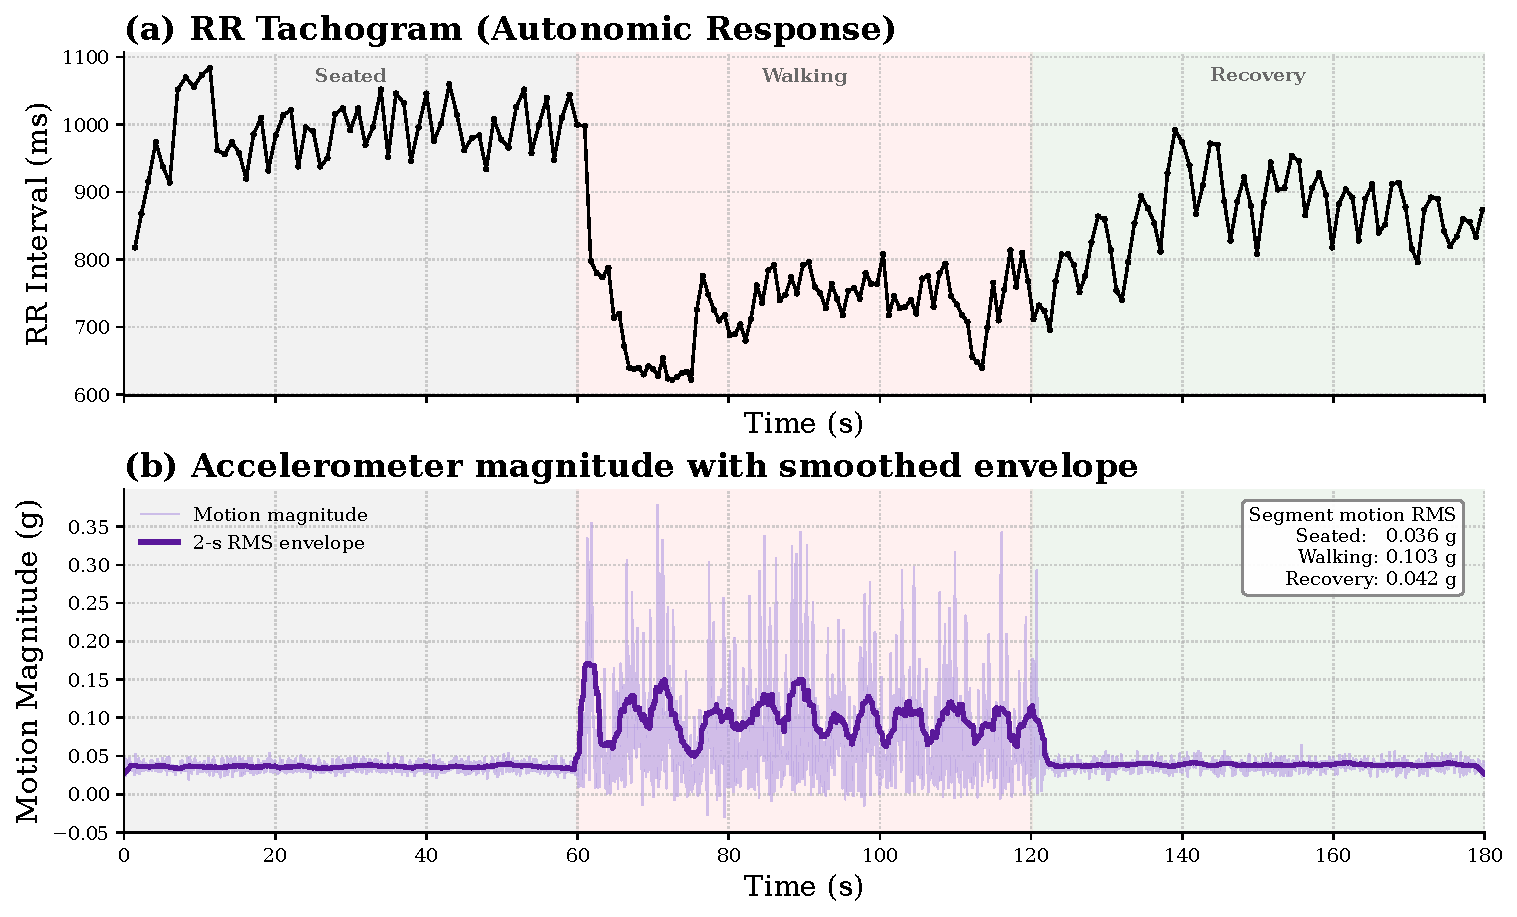
\includegraphics[width=0.92\linewidth]{nb04_fig05_e3_motion_crosscheck.pdf}
\caption{Walking challenge overview.
(a)~RR interval dynamics across seated baseline, walking, and
recovery. (b)~Accelerometer magnitude and 2-s RMS motion envelope.
Correlation between $|\Delta\text{RR}|$ and motion magnitude was
modest ($r = 0.26$).}
\label{fig:q3_walk}
\end{figure}

\begin{figure}[H]
\centering
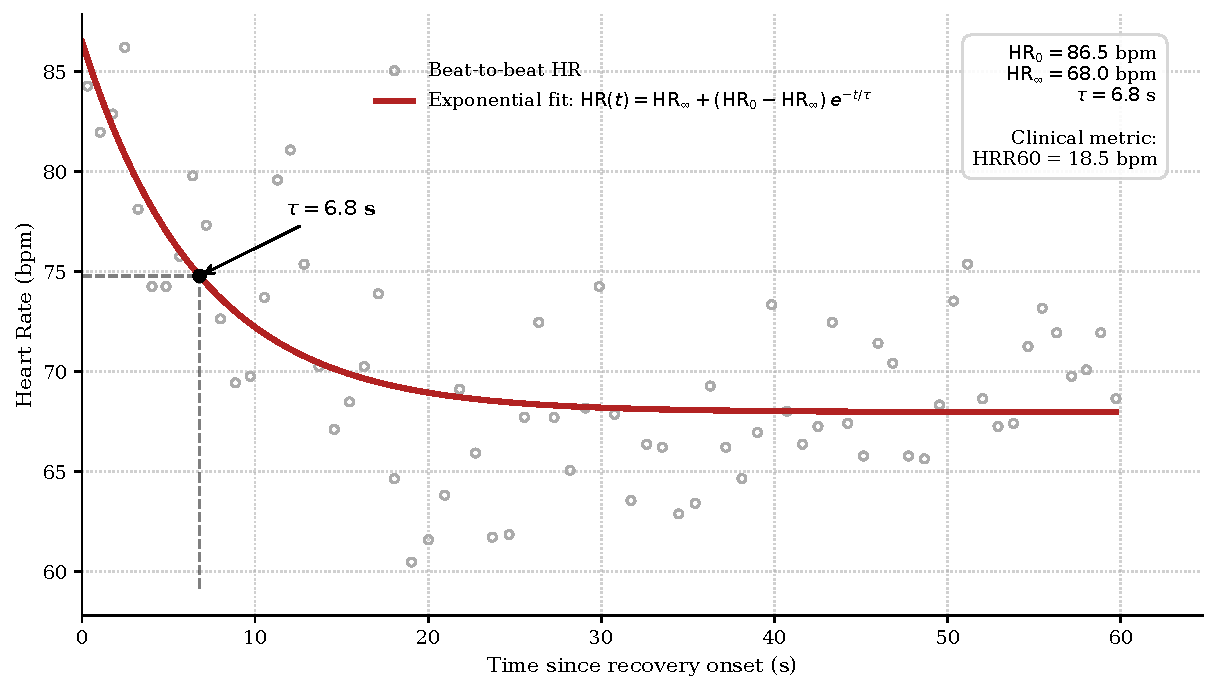
\includegraphics[width=0.92\linewidth]{nb04_fig03_e3_recovery_tau.pdf}
\caption{Post-walking heart-rate recovery. Beat-to-beat HR during the
60-s recovery segment fitted to a single-exponential decay
($\tau = 6.8$~s; HRR$_{60} = 18.5$~bpm).}
\label{fig:q3_recovery}
\end{figure}

% ------------------ Q4 ------------------
\subsection{Q4: Self-Designed Variation \textemdash{} Paced Breathing}

\begin{table}[H]
\centering
\caption{Paced-breathing HRV metrics across five metronome rates.}
\label{tab:q4}
\small
\setlength{\tabcolsep}{4pt}
\begin{tabular}{@{}lccccc@{}}
\toprule
                  & 12/min & 9/min & 6/min & 5/min & 3/min \\
\midrule
Expected (Hz)     & 0.200 & 0.150 & 0.100 & 0.083 & 0.050 \\
Measured (Hz)     & 0.203 & 0.148 & 0.102 & 0.086 & 0.047 \\
Mean HR (bpm)     & 59.4  & 57.0  & 60.2  & 59.9  & 58.1 \\
SDNN (ms)         & 48.7  & 78.0  & 91.3  & 95.9  & 131.4 \\
RMSSD (ms)        & 47.7  & 64.9  & 60.4  & 53.9  & 55.2 \\
LF/HF             & 0.22  & 0.84  & 11.55 & 17.45 & 17.46 \\
RR amplitude (ms) & 157   & 240   & 293   & 297   & 406 \\
\bottomrule
\end{tabular}
\end{table}

\textbf{Hypothesis.} Imposing slower respiration with a metronome will
shift the dominant respiratory peak in the RR spectrum to progressively
lower frequencies, crossing the conventional 0.15\,Hz LF/HF boundary as
breathing slows below 9 breaths/min. We also expected slow breathing to
increase RR-oscillation amplitude with little change in mean HR, given
that respiratory sinus arrhythmia couples breathing to vagal-mediated HR
modulation~\cite{taskforce1996}.

\textbf{Result.} Across the five paced conditions (Table~\ref{tab:q4};
Figs.~\ref{fig:q4_tach}, \ref{fig:q4_psd}, and~\ref{fig:q4_lfhf}), mean HR varied narrowly
(57.0--60.2\,bpm) while peak-to-trough RR amplitude grew from 157\,ms
(12/min) to 406\,ms (3/min). The dominant RR spectral peak closely tracked
the imposed breathing frequency at all five rates (absolute deviation
$\leq$0.003\,Hz; linear fit $R^{2}=0.998$). These observations were
consistent with the hypothesis: slower breathing increased RR oscillation
amplitude, shifted the respiratory peak leftward, and moved the peak
across the 0.15\,Hz boundary between the 12- and 9-breaths/min conditions.

\textbf{LF/HF observation.} As the respiratory peak crossed the LF/HF
boundary, the LF/HF ratio rose from 0.22 (12/min) to approximately 17.5
at the slowest rates, while RMSSD remained between 48 and 65\,ms across
all five conditions (Fig.~\ref{fig:q4_lfhf}). In this lab report, this
observation is reported descriptively without further mechanistic
interpretation. \emph{(A more detailed analysis is deferred to the Final
Project, which will examine LF/HF interpretability under respiratory-band
migration.)}

\begin{figure}[H]
\centering
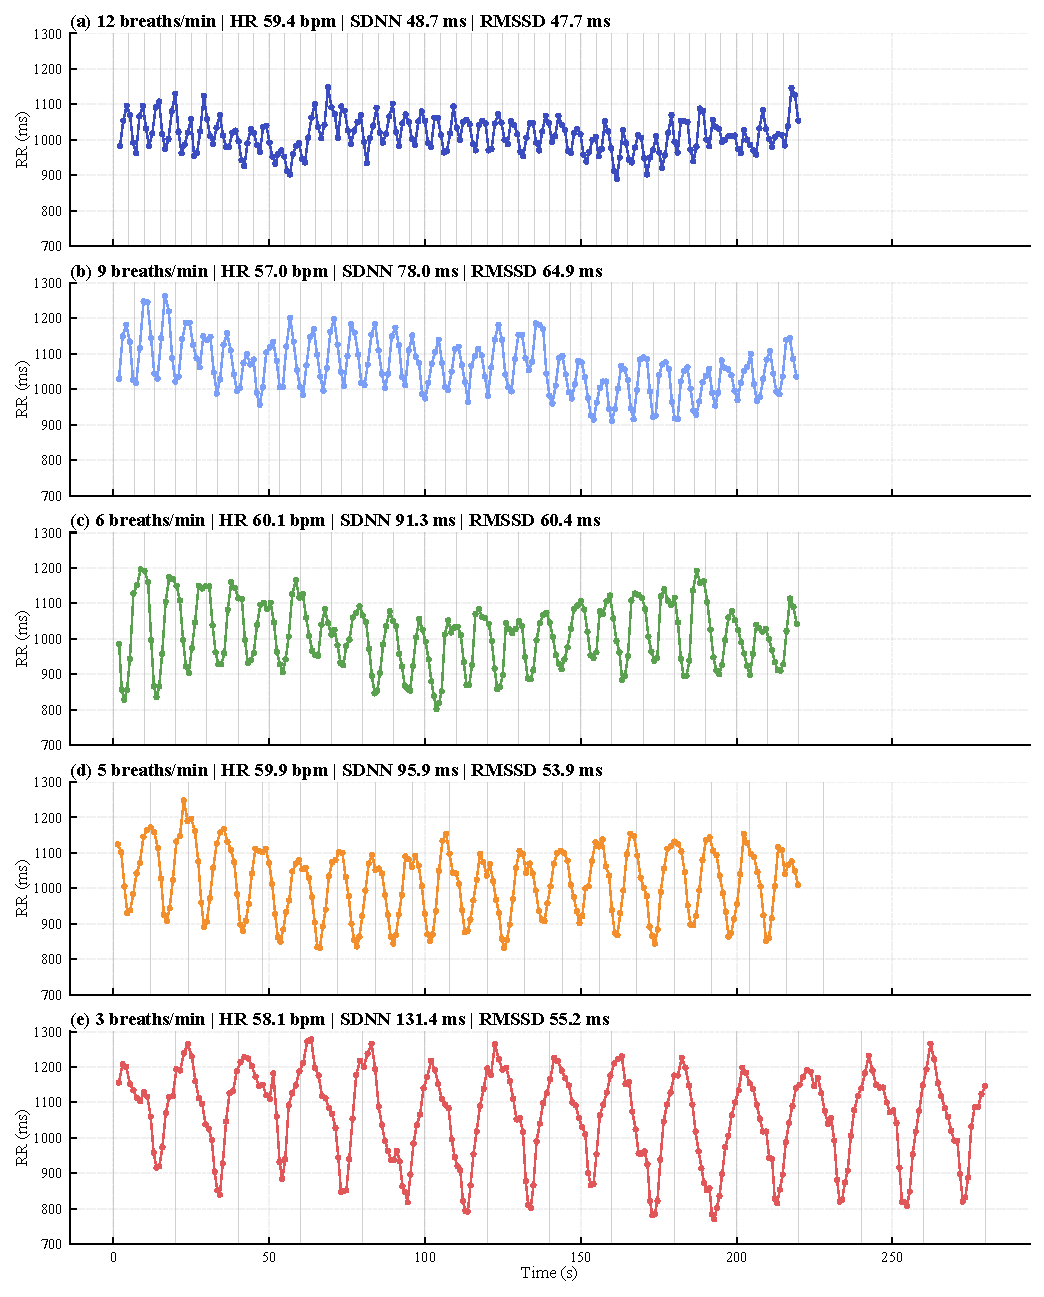
\includegraphics[width=0.92\linewidth]{nb05_fig01_e4a_tachograms.pdf}
\caption{RR tachograms during paced breathing at five metronome-guided
rates from 12 down to 3 breaths/min. Oscillation amplitude grows
monotonically as breathing slows; mean HR remains nearly constant. Grey
lines indicate cued inhalation onsets.}
\label{fig:q4_tach}
\end{figure}

\begin{figure}[H]
\centering
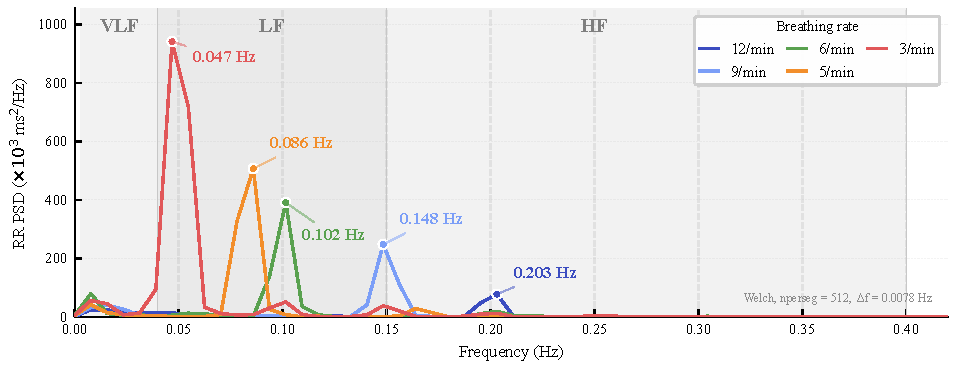
\includegraphics[width=0.88\linewidth]{hw05_q4_rr_psd_overlay_e4a.pdf}
\caption{RR-interval PSD overlay during paced breathing (band migration). Spectra use Welch's
method; window length and frequency resolution are annotated in-panel. Shaded bands follow Task Force
VLF/LF/HF definitions. The dominant peak tracks the imposed metronome rate and crosses the
0.15\,Hz LF/HF boundary between 12 and 9 breaths/min.}
\label{fig:q4_psd}
\end{figure}

\begin{figure}[H]
\centering
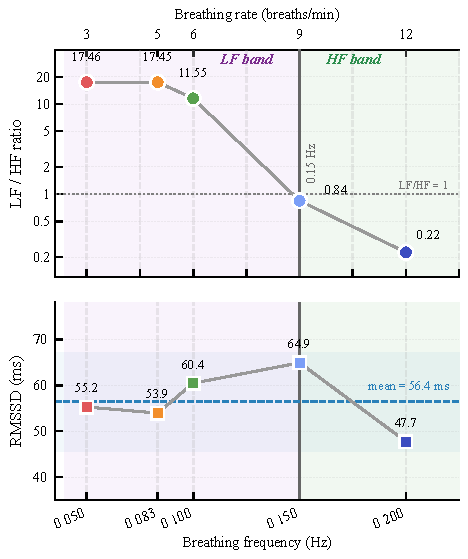
\includegraphics[width=0.55\linewidth]{hw05_q4_lfhf_rmssd_stacked_clean.pdf}
\caption{LF/HF ratio (log scale, upper panel) and RMSSD (linear scale, lower panel) vs.\
imposed breathing frequency during paced breathing. Shared shading marks Task Force LF/HF
bands; vertical line: 0.15\,Hz (upper axis: breaths/min). LF/HF rises sharply as the respiratory
oscillation migrates across the boundary, whereas RMSSD remains in a comparatively narrow range
(Table~\ref{tab:q4}).}
\label{fig:q4_lfhf}
\end{figure}

% ============================================================
\section{Discussion}

\textbf{Q1.} The supine--sitting--standing trajectory followed the
expected orthostatic HRV pattern: higher HR and lower RMSSD with
increasing postural challenge, accompanied by reduced HF
power~\cite{taskforce1996,shaffer2017}. The ECG-domain spectrum also
showed signal quality sufficient to resolve cardiac harmonics and a
respiratory-band peak.

\textbf{Q2.} The inspiratory--expiratory HR asymmetry suggests that lung
volume, in addition to respiratory cessation, contributed to the
breath-hold HR response in this participant. The substantial Trial-1
vs.\ Trial-2 divergence in the inspiratory condition shows how volitional
effort and anticipation can affect short-duration HRV measurements and
supports the use of repeated trials.

\textbf{Q3.} Walking elevated HR with rapid post-exercise recovery
($\tau = 6.8$\,s). However, the proximity of step frequency to the
cardiac fundamental and the low ECG--motion coherence suggest that
fine-scale HRV during walking should not be compared directly against
seated baselines. Mean HR and recovery kinetics remained interpretable,
but RMSSD during walking was motion-limited.

\textbf{Q4.} The paced-breathing experiment was consistent with the
hypothesis: imposed respiration shifted the dominant RR spectral peak
across the 0.15\,Hz LF/HF boundary, increased RR oscillation amplitude,
and left mean HR nearly unchanged. The LF/HF increase observed at slow
rates illustrates that band-defined indices can change substantially
without a corresponding shift in time-domain vagal markers. A more
detailed analysis of this asymmetry is left to the Final Project.

% ============================================================
\section{Conclusion}
The single-lead chest-patch ECG sensor captured HR and HRV changes across
postural loading, inspiratory--expiratory breath-hold, post-walking
recovery, and paced-breathing entrainment of the RR spectrum. Two contexts
required interpretive caution: motion artifact during walking and
respiratory-band migration of the LF/HF ratio during slow paced breathing.
These issues were condition-specific rather than obvious sensor failures,
and they motivate the broader LF/HF interpretability question addressed
in the Final Project.

% ============================================================
\begin{thebibliography}{9}

\bibitem{taskforce1996}
Task Force of the European Society of Cardiology and the North American
Society of Pacing and Electrophysiology,
``Heart rate variability: Standards of measurement, physiological
interpretation, and clinical use,''
\emph{Circulation}, vol.~93, no.~5, pp.~1043--1065, 1996.

\bibitem{makowski2021}
D.~Makowski \emph{et~al.},
``NeuroKit2: A Python toolbox for neurophysiological signal processing,''
\emph{Behav. Res. Methods}, vol.~53, no.~4, pp.~1689--1696, 2021.

\bibitem{pan1985}
J.~Pan and W.~J. Tompkins,
``A real-time QRS detection algorithm,''
\emph{IEEE Trans. Biomed. Eng.}, vol.~BME-32, no.~3, pp.~230--236, 1985.

\bibitem{shaffer2017}
F.~Shaffer and J.~P. Ginsberg,
``An overview of heart rate variability metrics and norms,''
\emph{Front. Public Health}, vol.~5, art.~258, 2017.

\end{thebibliography}

\end{document}
